With the goals of reusability and modularity in mind, LAD-4 was designed to use as many student researched and developed (SRAD) components as possible, with the exception of the use of a commercial/off-the-shelf (COTS) solid motor, which was determined to be the most economical and time-efficient strategy with respect to project development time. The rocket's aerostructure, recovery, and avionics systems were fully designed and fabricated by the team, using COTS parts only where necessary and within the framework of a student-developed system (e.g. a COTS barometric altimeter was used for apogee detection). These decisions were made in accordance with the mission goal of validating these components for future EUREKA flights. 
\newline\newline
The following figures illustrate the internal configuration of LAD-4. The top figure is a diagram from the OpenRocket simulator program and the bottom figure is a CAD model of the rocket and its systems with each component located precisely. The rocket was designed using a combination of commercial simulation software (e.g. OpenRocket) and a custom numerical calculator (section \ref{Trajectory Planning}) in order to establish important parameters such as stability, target mass, and predicted apogee. A CAD model of the rocket ensured that components would fit together during integration as designed and provided a basis for machining procedures (e.g. laser cutting).
\begin{figure}[H]
    \centering
    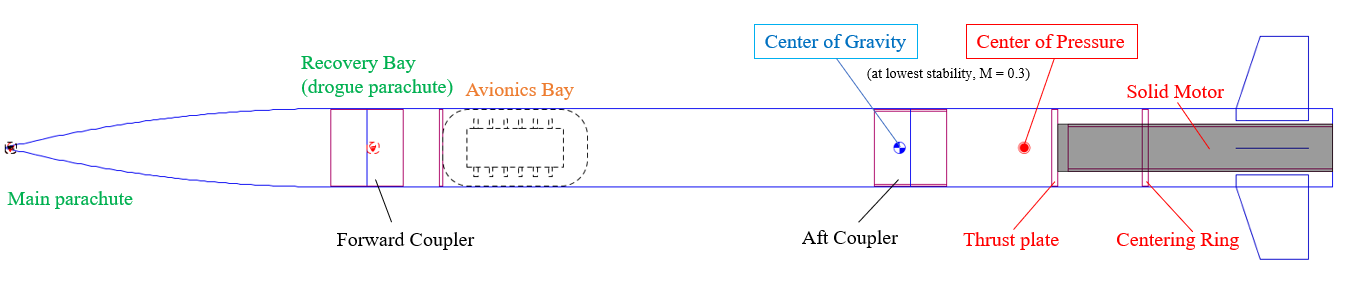
\includegraphics[width=\textwidth]{imgs/lad4skeletonfull.png}
    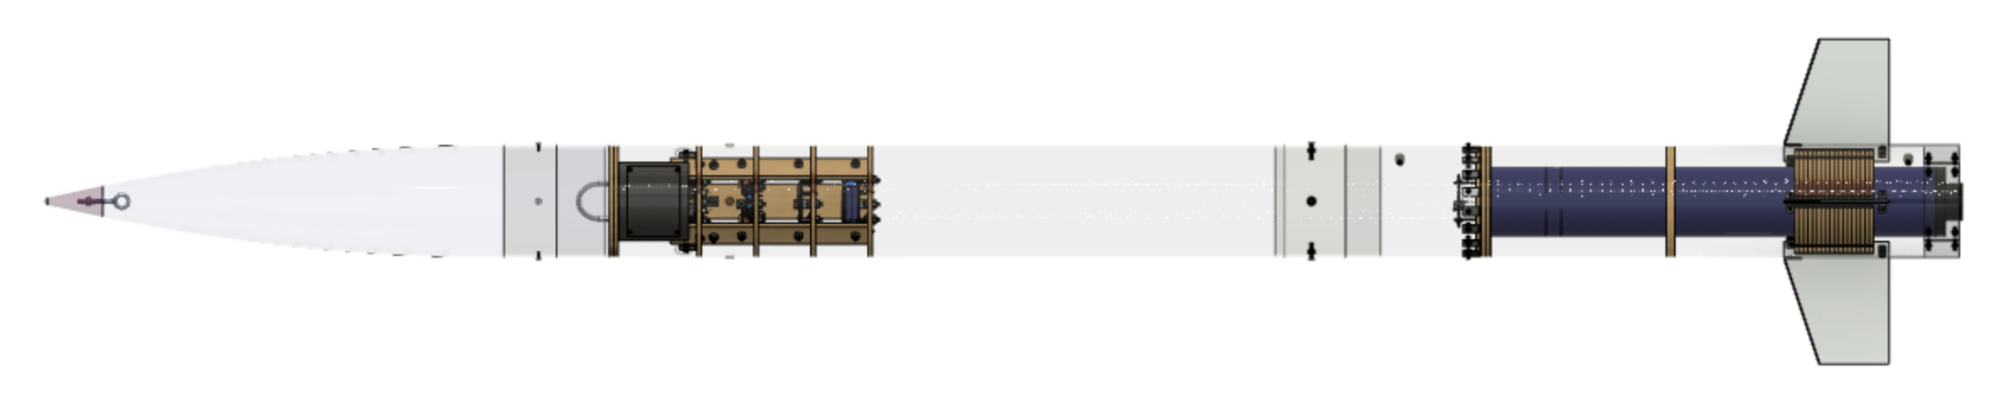
\includegraphics[width=\textwidth]{imgs/lad4internalfull.png}
    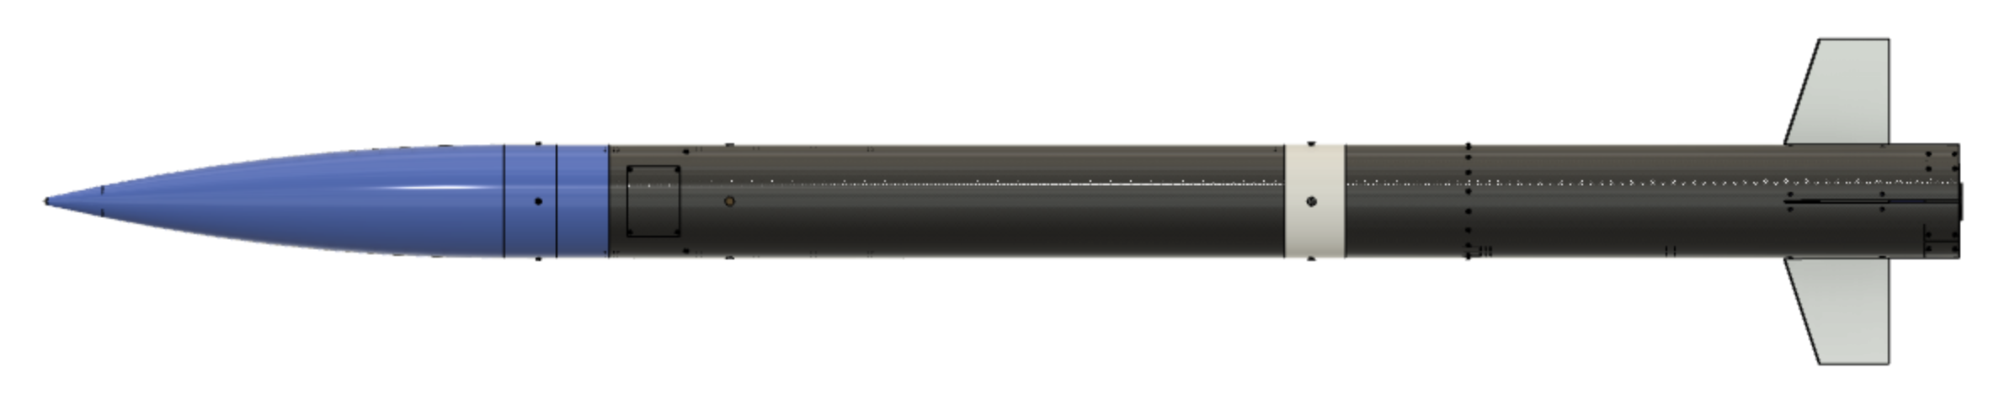
\includegraphics[width=\textwidth]{imgs/lad4airframefull.png}
    \caption{System Overview}
    \label{fig:systemoverview}
\end{figure}
The following table lists important top-level parameters for the rocket.
\begin{table}[H]
\begin{tabular}{|l|l|l|}
\hline
\textbf{Parameter}                                & \textbf{Value}                                       & \textbf{Unit}                                                    \\ \hline
Length                                            & 90                                                   & inches                                                           \\ \hline
Nominal outer diameter                            & 6.5                                                  & inches                                                           \\ \hline
Dry mass                                          & 13                                                   & kilograms                                                        \\ \hline
Theoretical (calculated) apogee                   & 13 142                                               & feet                                                             \\ \hline
Theoretical (calculated) maximum speed            & \begin{tabular}[c]{@{}l@{}}1.07\\ 356.6\end{tabular} & \begin{tabular}[c]{@{}l@{}}Mach\\ meters per second\end{tabular} \\ \hline
Motor impulse, total (manufacturer specification) & 7673                                                 & newton-seconds                                                   \\ \hline
\end{tabular}
\end{table}
\subsection{Airframe}
The LAD-4 airframe consists of a nosecone and two main body tubes, which house four main sections. The \textit{recovery bay} is situated in the aft portion of the nosecone and the forward portion of the forward tube, sealed by the forward pressure bulkhead. Aft of the bulkhead is the \textit{avionics bay}, which consists of the apogee detection and charge deployment system, a custom data-logging system, and a radio transmitter module. In the aft airframe tube, the thrust plate sits forward of the motor housing, which retains and centers the \textit{motor assembly}. The \textit{fin can section}, which contains the architecture to secure and stabilize the fins, is located at the aft end of the rocket.
\subsubsection{Nosecone}
LAD-4 features a fiberglass nosecone manufactured in-house by team members. Fiberglass was chosen to maintain radio transparency, with the avionics bay in close proximity.
\begin{figure}[H]
	\centering
	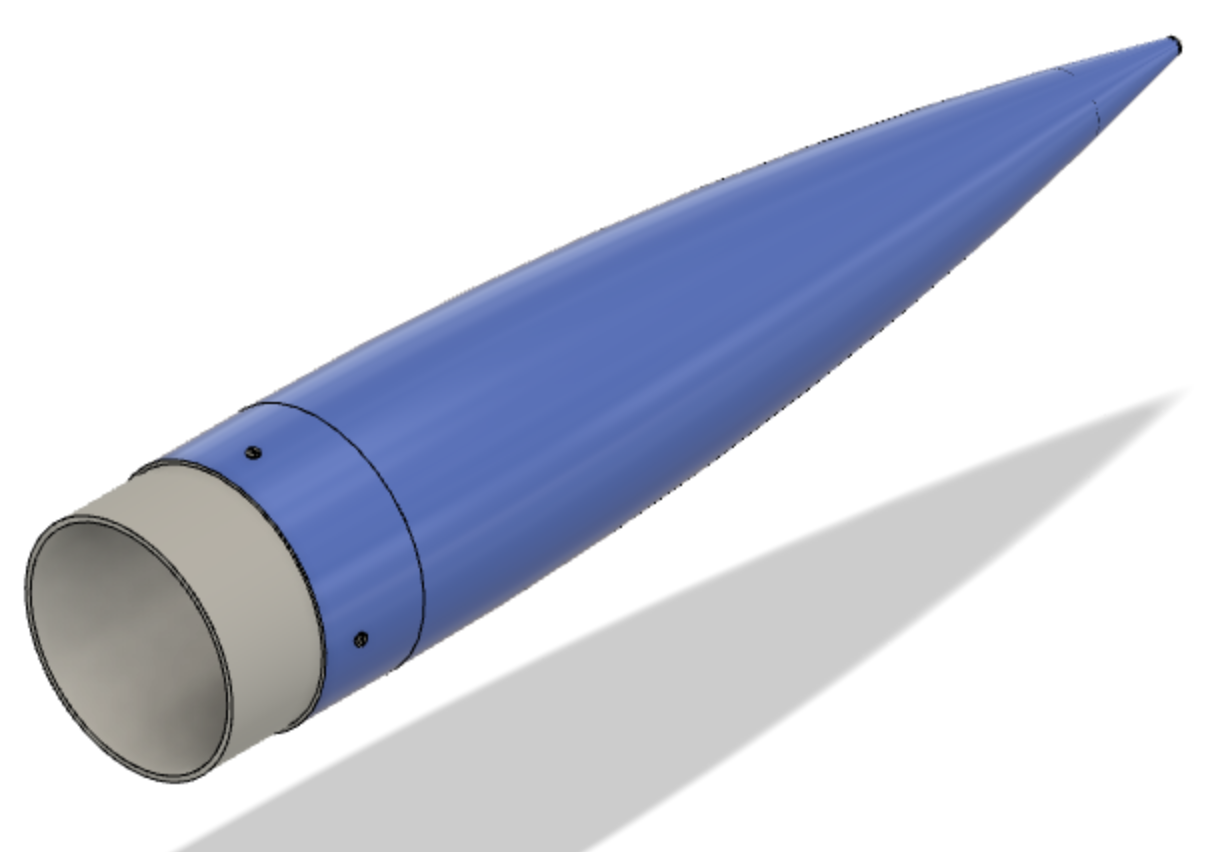
\includegraphics[width=3.5in]{imgs/nosecone.png}
	\caption{Nosecone}
	\label{fig:nosecone}
\end{figure}
\subsubsection*{Design}
The nosecone of the rocket was a tangent ogive shape with a total length of 30 inches, which includes a 3-inch straight section built in for additional recovery equipment space. As the principal criterion for nosecone design was aerodynamic, studies of drag at various speeds were done with multiple ogive designs, as well as conical and power-law designs. It was determined that the tangent-ogive shape was most appropriate for the transsonic range of LAD-4.
\subsubsection*{Manufacturing}
The nosecone was made using two identical negative molds, each the shape of half of the nosecone. The two molds were produced out of medium-density fiberboard (MDF) on a Shopbot CNC mill. 
\begin{figure}[H]
	\centering
	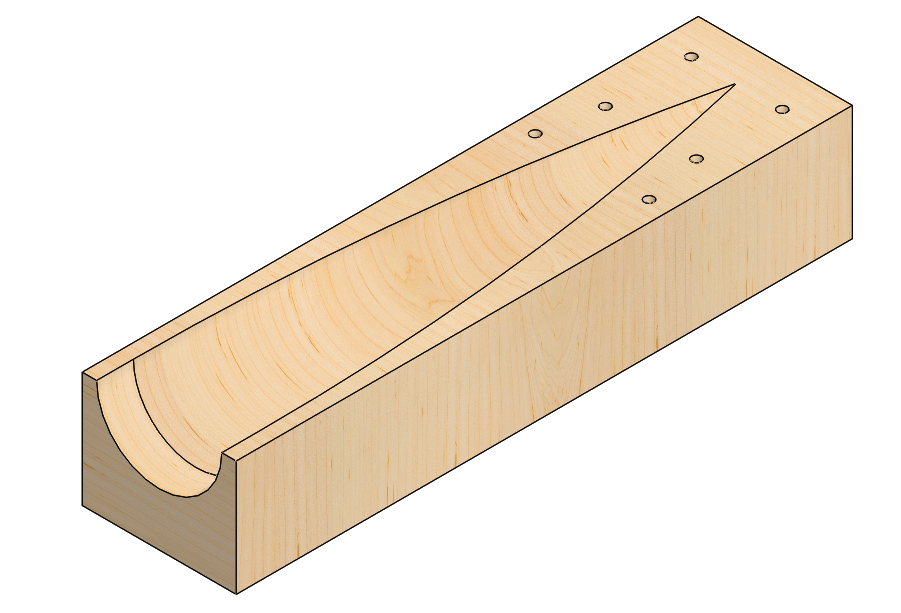
\includegraphics[width=3.5in]{imgs/noseconemoldhalf.png}
	\caption{Nose Cone Mold Half}
	\label{fig:noseconehalf}
\end{figure}
The molds were prepared with two coats of paste wax (``turtle wax'') and two coats of polishing wax. After the wax dried according to the manufacturer’s instructions, the nosecone was laid up with seven layers of E-glass fiberglass and TAP Plastics epoxy resin. The layers were thoroughly saturated and applied in quick succession. Fiberglass “templates” for each layer were cut out in the shape of a triangle prior to the layup process to save material. 	The two halves were joined together using wooden dowels as alignment pins in the 6 holes visible in Figure \ref{fig:noseconehalf}. After the halves were aligned, fiberglass patches were applied along the interior seam between each mold half, followed by a slurry of epoxy resin and chopped fiberglass fibers. The nosecone was then allowed to cure according to the epoxy manufacturer’s directions for a minimum of 24 hours.
\newline\newline
After the epoxy cured, the nosecone was removed from the mold. After removal, a number of small surface imperfections were observed on the cone. Most notably, there was a small ridge along the line of the seam between the mold halves. The ridge and other surface defects were sanded, filled in using Bondo body filler, and finished with successive rounds of sanding and filling until a smooth, uniform surface finish without ridges, dents, or other substantial imperfections was achieved. The inside of the nosecone was cleaned using a wire brush attached to a power drill, and the uneven bottom edge of the nose cone was finished on a tile saw to achieve a true bottom mating surface against the upper airframe tube.
\subsubsection*{Eye-Bolt}
The tip of the nosecone was filled to a height of 4 inches with a fiberglass-resin slurry, and an eye-bolt was submerged into the wet slurry and suspended in place such that when the resin fully cured, the “stem” of the eye-bolt was entombed in hardened slurry and the “eye” of the eye-bolt was fully exposed. The “eye” served as a hard point for the attachment of the nose cone to the parachute and recovery gear.
\subsubsection{Body Tubes}
The two fiberglass/carbon-fiber body tubes of the rocket were also manufactured by team members using continuous fiber sheets. The rocket features a monocoque load-carrying aerostructure, which does not require the use of longerons to provide stiffness or strength.
\subsubsection*{Design}
Because of the high aspect ratio and low thickness of the airframe, the principal failure modality of the body tubes to be considered is buckling. The state of loading on the airframe consists of two major sources of compressive stress: aerodynamic drag and an internal force from the motor, which is passed through to the airframe via a thrust plate. Thus the maximum total stress occurs at the end of the motor burn, where the dynamic pressure is at a maximum (the point of “max $q$”). The dynamic pressure over time, calculated using motor parameters and the manufacturer’s thrust curve, is shown in the following figure.
\begin{figure}[H]
	\centering
	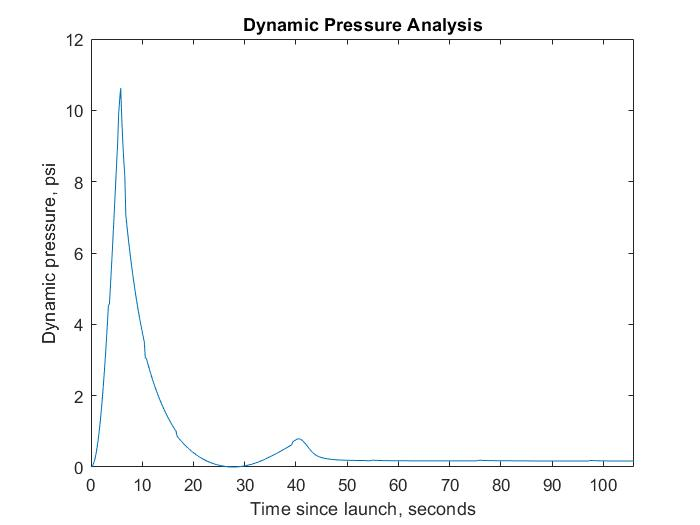
\includegraphics[width=3.5in]{imgs/dynamicpressurevtime.jpg}
	\caption{Dynamic pressure on the rocket as a function of time. The peak dynamic pressure occurs at the end of motor burn, around 5.7 seconds into the flight.}
	\label{fig:dynamicpressure}
\end{figure}
LAD-4’s airframe is composed of bidirectionally-woven fiberglass, chosen for its high specific strength and stiffness, as well as its lower cost compared to other materials used in fiber-reinforced polymer composites such as carbon fiber. An analysis of the critical buckling load on an airframe tube was conducted to determine the amount of material needed for the airframe in order to withstand the maximum dynamic pressure with a minimum safety factor of 2.0. Though a degree of variability is introduced in the manual production of airframe tubes, the properties of the laminate were determined using the laminated plate theory described by Gibson [\href{example.com}{citation}], and the necessary thickness was calculated using Euler’s formula for beam buckling. In all, four layers of fiberglass and one layer of carbon fiber were used; the last layer of fiberglass was substituted for a layer of bidirectional carbon fiber in manufacturing. The main body tubes consisted of two sections laid up independently: one 48-inch section and one 38-inch section. The nominal inside diameter of the tubes was 6.3”, and the nominal outside diameter of the tubes was 6.5”. As a final step in the design process, the rocket was mocked up in a simulation program and evaluated for its stability. The results are plotted below. 
\begin{figure}[H]
	\centering
	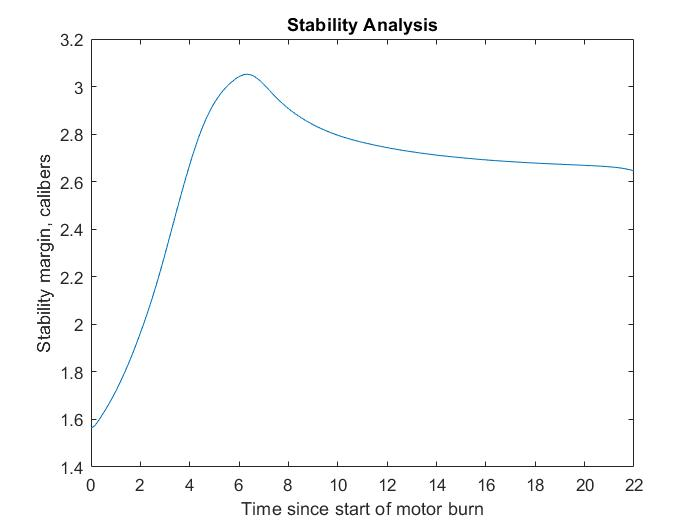
\includegraphics[width=3.5in]{imgs/stabilityanalysis.jpg}
	\caption{Stability analysis obtained from a simulation program \text{(OpenRocket)} and plotted.}
	\label{fig:stability}
\end{figure}
In the duration of flight before apogee is reached and the drogue parachute is deployed, the stability was determined to be within a safe envelope (greater than 1.5 calibers and less than 6 calibers).
\subsubsection*{Manufacturing}
The body tubes were laid up by hand using a wet layup process. A cardboard mailing tube with a 6'' outside diameter was used as a central mandrel, onto which a layer of mylar was wrapped tightly to aid the airframe removal post-cure. The mandrel was wetted with epoxy, and the woven fiberglass cloth, pre-cut to size by layer, was wrapped onto the mandrel and subsequently wetted out. This process was repeated layer by layer for the four fiberglass layers and one carbon fiber layer, rotating the seam by approximately 60 degrees each time to prevent ridges. After the last (carbon fiber) layer was wetted out, peel-ply film was wrapped tightly around the layup to create a consistent surface finish by soaking up excess epoxy. The tube was then left to cure for a minimum of 24 hours, as given in the epoxy manufacturer’s guidelines.
\newline\newline
After the epoxy was fully cured, the body tube exteriors were repeatedly sanded down and re-wetted with epoxy until the surface finish was smooth. Increasingly finer-grit sandpaper was used, up to 3000 grit sandpaper for the final pass. The ends of the airframe tubes were then removed using the tile saw, such that each tube had two clean, perpendicular ends. This resulted in a slightly shorter overall length of each tube; the final airframe tubes had lengths of 45 inches and 35 inches. 
\subsubsection*{Static port holes}
During the final assembly process, four static port holes of diameter 0.25” were drilled in the airframe near the Stratologger module to normalize the internal pressure with the atmospheric pressure, enabling the barometric altimeter to function properly.
\subsubsection*{Access panel}
An access panel was created in the forward body tube for access to the Avionics bay after integration. The access panel was a 1.5” by 2.5” cutout in the airframe, secured via rivnuts, with a backing plate installed within the airframe. The backing plate was made using a scrap section of 6”-diameter carbon fiber tube, and permanently affixed to the airframe with epoxy. The access panel could then be removed and reattached to the backing plate freely.
\begin{figure}[H]
	\centering
	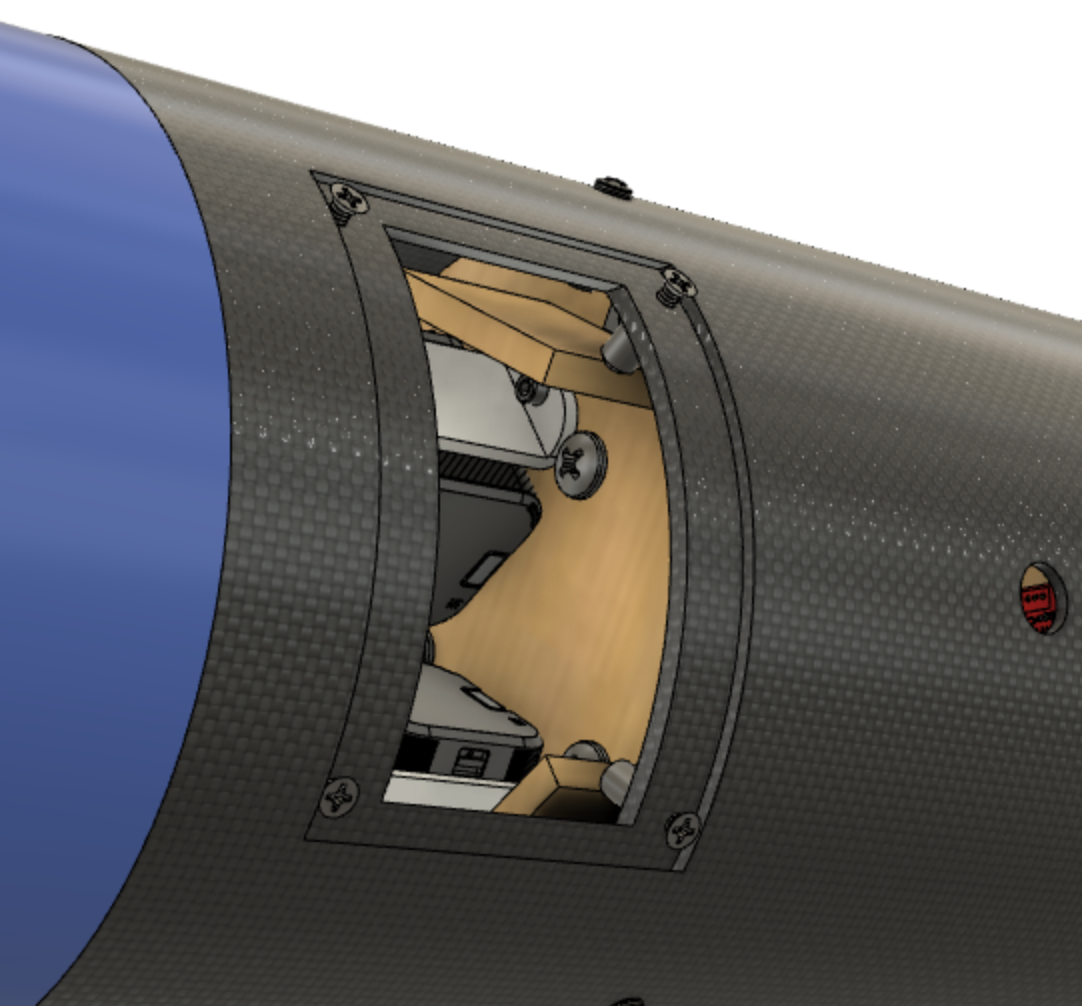
\includegraphics[width=4in]{imgs/accesspaneldetail.png}
	\caption{Access Panel detail. Aft of the access panel, a camera hole is visible.}
	\label{fig:accesspanel}
\end{figure}
\subsubsection*{Fin slots}
Fin slots, extending 9” from the aft end of the airframe, were created using a router and a custom laser-cut plywood jig. The rectangular jig consisted of a box with a missing side for the excess length of tube to protrude through as well as a removable top with a 0.13” by 9” slot for the router bit to stick through. The router was pushed along a groove on the removable top parallel to the slot and cut the tube beneath. The jig also included a square frame press fitted on the protruding end of the tube to ensure that the slot centerlines were 90 degrees apart.
\subsubsection{Coupler Sections}
There are two coupler sections used to connect the three manufactured portions of the airframe. Both coupler sections had a phenolic-like core, made of 6”-diameter Blue Tube (Always Ready Rocketry, Inc., Mt. Vernon, WA) cut to length. The Blue Tube was inserted into 6”-inner-diameter mailing tubes and epoxied into place, forming a bilayer structure. The outside of the mailing tubes were then sanded down until they were able to be inserted the correct distance into the body tubes. The \textit{forward coupler} was epoxied onto the aft portion of the nosecone and is used to bridge the nosecone and the forward body tube. The forward coupler is attached to the forward body tube using three nylon bolts, designed to shear at apogee and eject the nosecone. The \textit{aft coupler} attaches the forward body tube to the aft body tube and is bolted into both composite skins. 
\subsubsection{Fins}
LAD-4 is equipped with four metal fins, made from 6061 aluminum sheets of 1/8" thickness.
\subsubsection*{Design}
Aluminum was chosen as the fin material due to its high specific stiffness and for its ability to be machined consistently. The team experimented with all-carbon fiber fins but found that variance in the layup process resulted in nonuniform fins. The aluminum fins, manufactured using a laser cutter, have the profile shown below, with a 6” span, a 2” sweep distance, and a 6” root chord. The bottom 1” of the fin, below the slot, is completely internal and provides contact surface area for the fin can assembly. The slot in the forward section of the fin slides into a corresponding slot made in the airframe, and locks the fin into place, preventing rotational motion. Additionally, the leading edge of each fin is bevelled to a 45 degree angle to reduce the induced drag.
\begin{figure}[H]
	\centering
	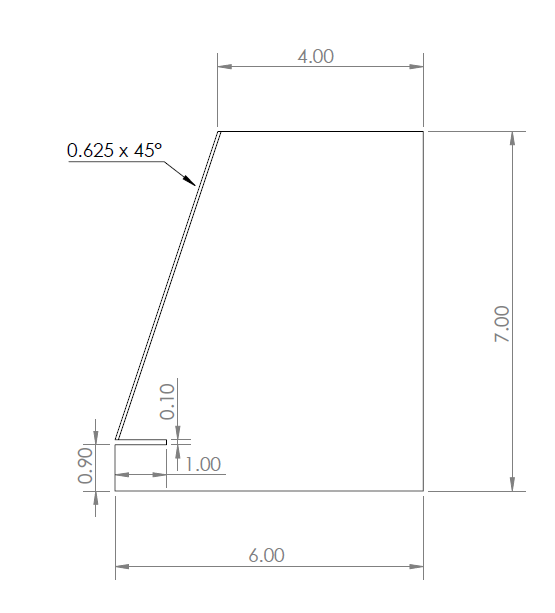
\includegraphics[width=4in]{imgs/fingeo.png}
	\caption{Fin design geometry. All dimensions are in inches; fin thickness is uniformly 0.125''.}
	\label{fig:fingeo}
\end{figure}
A principal concern in fin design is aeroelastic flutter, a phenomenon that occurs above a critical \textit{flutter velocity} whereby any transverse oscillations on the fin are amplified rather than damped, leading to the catastrophic failure of the fin and extreme instability in subsequent flight. The flutter velocity is dependent largely on the fin geometry and material. Using the equation provided by Howard (2011), and the fin geometry given, the flutter speed was calculated to be in excess of Mach 2, much higher than the predicted maximum velocity in flight. The designed fins were determined to be safe against flutter with a factor of safety of 1.90.
\subsubsection*{Manufacturing}
The fin profile was drawn using AutoCAD and the DXF file was sent to a Fablight laser cutter for manufacturing. A laser cutter was used to ensure consistent dimensions across all fins and to minimize the kerf distance. The bevel was done freehand using a belt sander. After the final assembly of the rocket, the fins were cleaned and polished using a 6000 grit whetstone to achieve a smooth finish.
\subsubsection{Fin Can}
In accordance with the project goal of flying the LAD-4 airframe several times, the fin retention system is designed to be completely modular. Consequently the fin can section allows for the simple replacement of a single damaged fin (e.g. from a rough landing) between flights. This means that the fins are not permanently bonded to any portion of the airframe. In previous LAD rockets, permanent fin fillets were created using a carbon fiber slurry and used to bond the fins to the airframe, followed by a tip-to-tip layup. Though the fillet-layup method is effective in adding the needed strength and stiffness to the fins, it effectively renders the aft body tube and fins as one complete unit. In LAD-4, a new, completely modular \textit{fin can} was designed and manufactured to allow for the same structural stability with the added benefit of replaceability. 
\subsubsection*{Design}
The design goals of the fin can section were: (a) to retain each fin and provide structural stability against translational motion in any dimension, (b) prevent a bending moment about the fin root that could lead to dangerous flutter conditions, and (c) allow for the easy removal and replacement of a single damaged fin and avoid any sort of permanent bonding. To strengthen the fin-fuselage attachment, a through-wall mounting system is used: a set of wooden centering rings, attached around the motor housing, mate with the fins, themselves attached to the motor housing via L-brackets. Together with the centering rings, a slot cut into the leading edge of each fin which mates with a slot cut into the airframe ensures alignment is exact and repeatable, while retaining the fin against circumferential and longitudinal motion. The L-bracket system provides a pre-load against a bending moment, damping oscillations in the fin. The entire assembly can be assembled independent of the rest of the airframe, slid in via the airframe slots, and secured by tightening bolts into the L-brackets and rivet nuts on the airframe.
\begin{figure}[H]
	\centering
	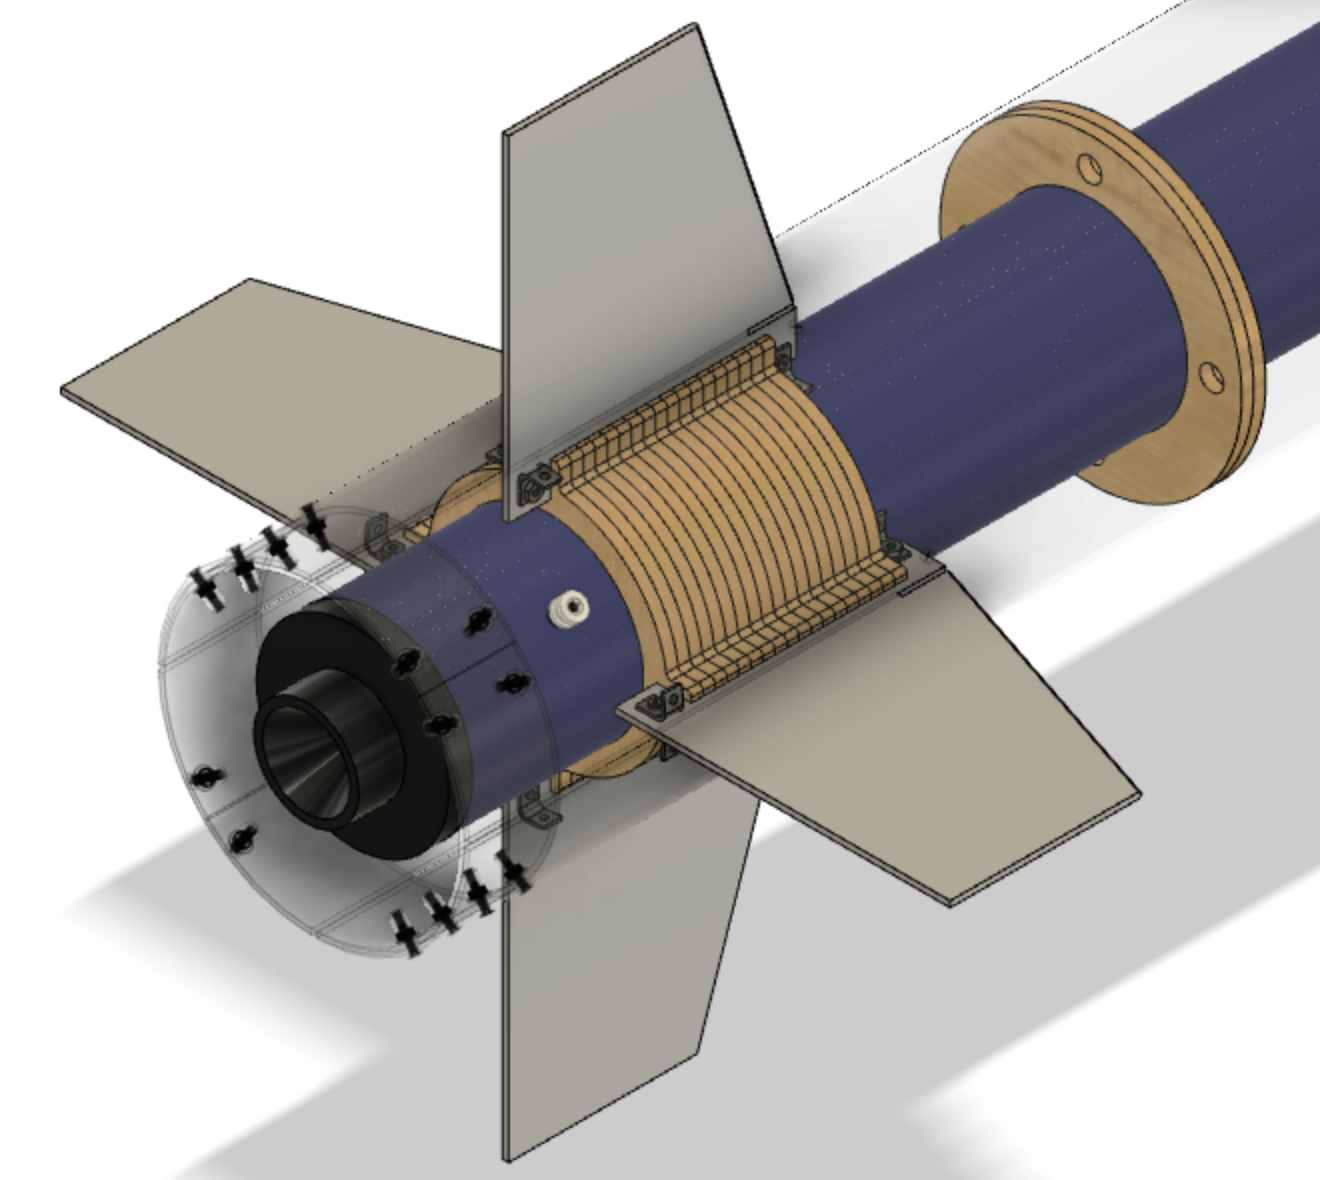
\includegraphics[width=4in]{imgs/finattachmentdetail.png}
	\caption{Detail of Fin Can and Fin Attachment System}
	\label{fig:fincan}
\end{figure}
\subsubsection*{Manufacturing}
The eighteen wooden rings were manufactured by laser cutting out \sfrac{1}{8}” plywood. The wooden rings were then attached to the motor housing one at a time with the first ring being 6\sfrac{1}{2}'' from the bottom of the housing. A single layer of epoxy was applied in between each ring and the motor housing. Once all the rings were attached, two layers of carbon fiber were applied to the outside of the wooden ring assembly, across all of the rings. The L-brackets were attached first to each fin in a designated position, so that they could be tightened upon integration of the fin can section.
\begin{figure}[H]
	\centering
	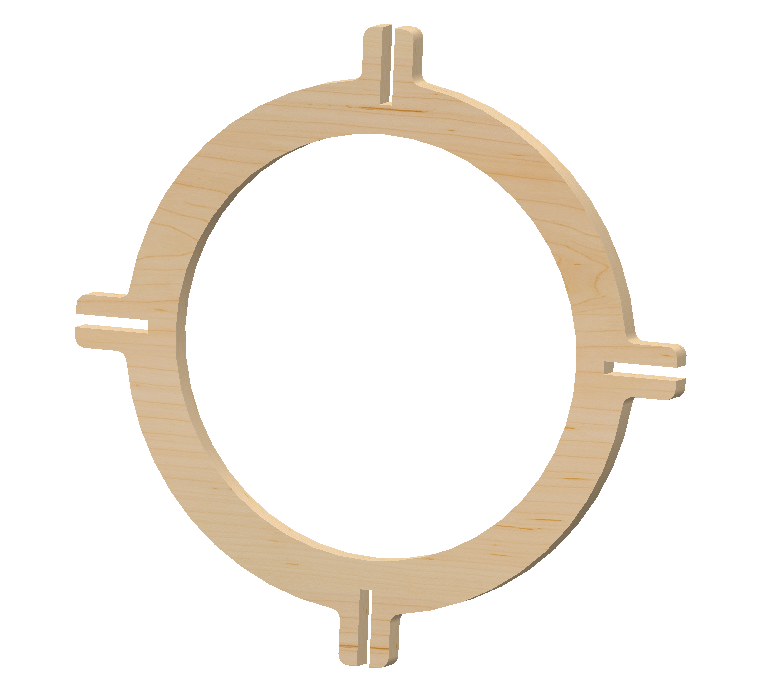
\includegraphics[width=2in]{imgs/retentionring.png}
	\caption{One of eighteen wooden fin alignment and retention rings.}
	\label{fig:retentionring}
\end{figure}
\subsubsection*{Integration}
First, the fin can assembly was created by inserting all 4 fins into the grooves formed by the wooden rings. Then, the entire assembly is attached to the airframe by aligning the fins to the slots made in the aft body tube and sliding the fins such that the slots in the fins interlock with the slots in the aft body tube. Once the fin can was seated, the L brackets on the fin can were secured to the rivnuts in the airframe.  Beneath the fins, small composite ‘band-aids’ were mounted to the inside of the aft body tube at the aftmost end to stabilize sections between the fin slots. The ‘band-aids’ were small, rectangular portions cut out of a previously-constructed 6”-diameter airframe tube, so that they were pre-formed into the correct radius.
\begin{figure}[H]
	\centering
	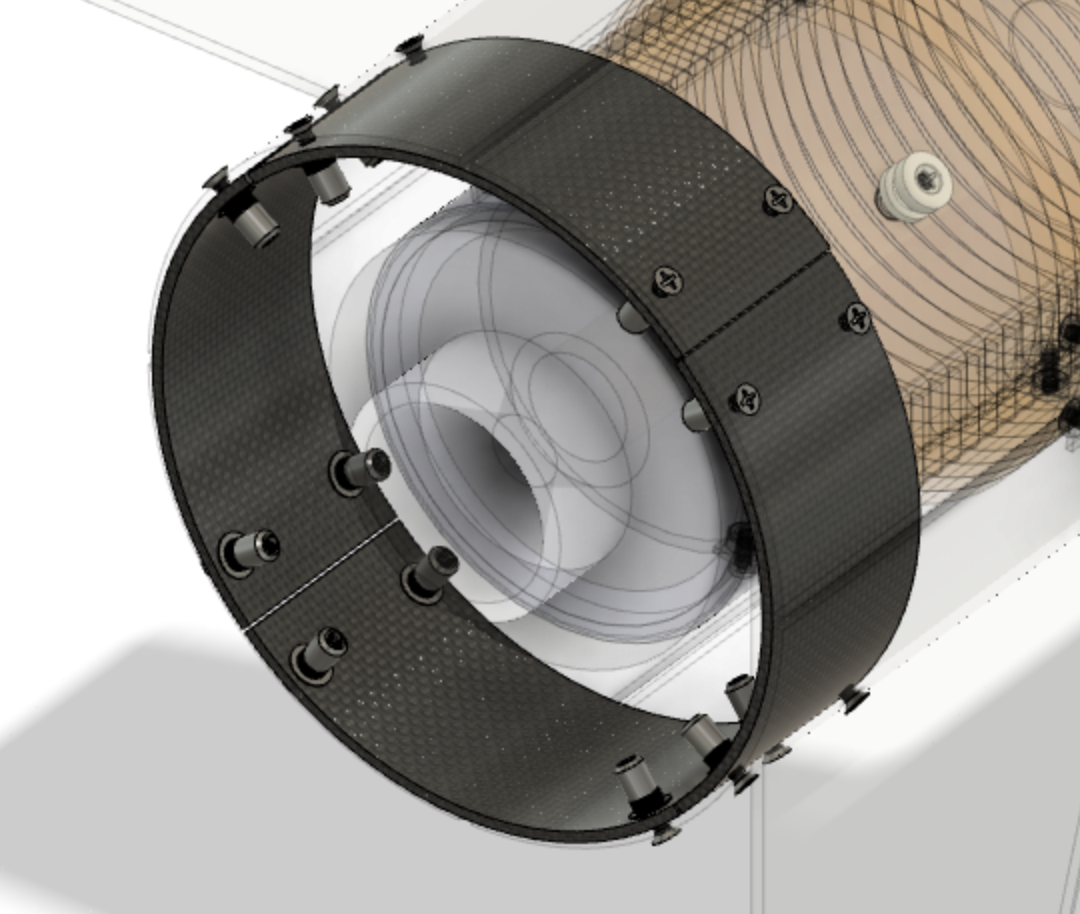
\includegraphics[width=3.5in]{imgs/finslotdetail.png}
	\caption{Fin Slot ``Band-Aids''}
	\label{fig:finslot}
\end{figure}
\subsubsection{Bulkheads}
\subsubsection*{Thrust plate}
The thrust plate, responsible for transferring loads from the engine through to the airframe, was created from two \sfrac{1}{4}” plywood discs glued together with four layers of fiberglass and one layer of carbon fiber laid up on both sides for a total of 10 composite layers. The thrust plate was attached to the airframe at a position that allowed contact with the motor assembly.
\begin{figure}[H]
	\centering
	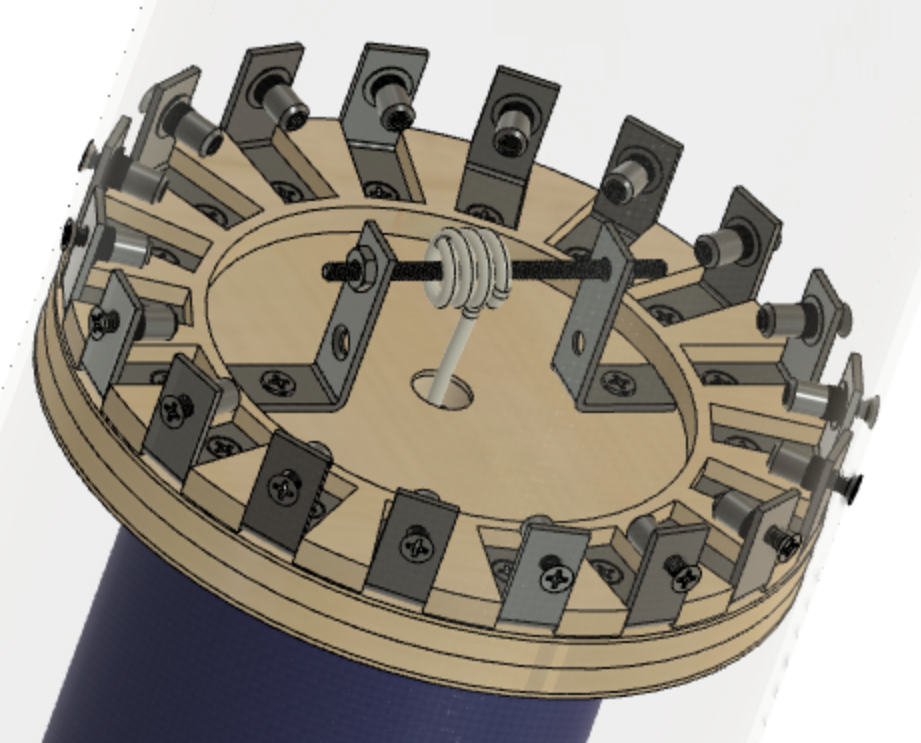
\includegraphics[width=3.5in]{imgs/thrustplatedetail.png}
	\caption{Thrust plate detail, showing the motor retention system (center). The eighteen bolts around the circumference of the thrust plate are screwed through the airframe, securing the thrust plate in place. In the center, a nylon rope secures the motor to the thrust plate, preventing it from falling out of the rocket.}
	\label{fig:thrustplate}
\end{figure}
\subsubsection*{Motor retention}
For the purposes of retaining the motor and motor housing within the airframe after it had fired, a length of paracord was tied to an eye-bolt threaded to the top of the motor, passed through a small hole drilled in the thrust plate, and tied to a threaded rod set off from the thrust plate.
\subsubsection*{Attachment to airframe}
For the purposes of thrust transfer to the airframe, the thrust plate was attached to the airframe using a set of eighteen L-brackets, which were bolted into the thrust plate itself.  For alignment purposes, in the other hole of each L-bracket, a threaded insert (rivnut) was installed. This allowed a bolt to be threaded in from the outside of the airframe in a secure manner.  A laser-cut wood piece was attached to the top of the thrust plate to align the L-brackets.
\subsubsection*{Pressure plate}
The pressure plate served as a bulkhead between the deployment charge/recovery compartment and the avionics bay. It is necessary for the purposes of (a) protecting the avionics bay and the rest of the rocket from the heat and forces of the explosive charge, and (b) to facilitate the buildup of pressure within the recovery compartment that would fracture the shear pins and eject the nosecone. It also served as the forward stop for the avionics bay. The pressure plate had a core made of \sfrac{1}{4}"-thick wood and was laid up with four layers of fiberglass on each side. No carbon fiber was used to lay up the pressure plate to ensure that radio transmission was possible from the avionics bay to the exterior of the rocket. A small hole was drilled in the pressure plate for the passage of wires between the avionics bay and the charges. 
\newline\newline
Additionally, a U-bolt was attached to the forward side of the pressure plate. This U-bolt served as the hard point on the airframe for the drogue parachute. The pressure plate was constructed on its own and epoxied into the airframe using a fiberglass-resin slurry that created a fillet around the edge of the pressure plate.
\subsection{Propulsion}
Inasmuch as the primary project goal of LAD-4 is to provide a robust vehicle for iterative validation flights of avionics and recovery system components, the propulsion system was designed to use a COTS solid motor. The decision to use a commercially available motor drastically reduces development cost and time, and provides a reliable propulsion source for each flight, reducing the number of variables in the system. 
\subsubsection{Propulsion System Overview}
The propulsion system on the maiden flight of LAD-4 uses an Aerotech M1340W-PS solid motor, which consists of three individual ammonium-perchlorate composite propellant (APCP) grains. The mass of the propellant is 4.036 kg, and the motor provides an average thrust of 1346.14 newtons during a 5.7-second burn time. The motor was assembled two days before launch, and integrated into the rocket during final assembly. The included electronic motor starter was used to ignite the engine on the launchpad. The M1340W-PS motor results in a thrust-to-weight ratio of 7.62 on launch, and results in a vehicle speed of 27.89 m/s (91.52 ft/s) off the launch rail, sufficient to withstand significant wind forces. 
\newline\newline
The following figure plots the thrust of the motor over time [\href{http://www.thrustcurve.org/}{source}].
\begin{figure}[H]
    \centering
    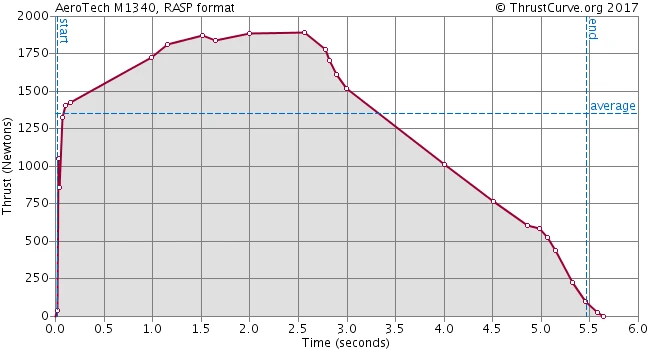
\includegraphics[scale=0.6]{imgs/thrustcurvesolid.png}
    \caption{Thrust curve for the Aerotech M1340W-PS solid motor.}
    \label{fig:thrustcurve}
\end{figure}
Though an Aerotech M-class motor was used on the first flight, the rocket is capable of integrating with any other 98mm-diameter motor system. This provides the ability to tailor the rocket’s performance (speed and altitude) to the specific goals of the testing performed on that flight. 
\subsubsection{Trajectory Planning}\label{Trajectory Planning}
A comprehensive numerical “flight simulator”, or trajectory planner, was created to accurately estimate critical flight parameters during manufacturing and testing, using a set of predetermined parameters (independent variables). It is based on a simple premise: model the flight of a rocket only in one dimension and using basic kinematic equations. By using a small time-step (0.2s), these kinematic equations can achieve sufficient granularity to create close approximations of the rocket's flight capabilities and final apogee. 
\newline\newline
On a more detailed level, the simulator required thrust, drag, gravity, and mass data. From these basic requirements, the need for atmospheric density data as a function of altitude, detailed drag properties of the rocket over a wide speed range, and a reliable model relating thrust, altitude, and time were necessary. Once these basic features were in place, more interesting calculations such as dynamic pressure, acceleration ($G$) load, and aerodynamic stability became possible. The calculation of these parameters heavily informed the design of the airframe and recovery systems, allowing weight and cost to be minimized where possible. For example, once a motor with a known thrust curve is chosen, the expected apogee of the rocket and the maximum loading condition on the airframe can be determined.
\newline\newline
The one-dimensionality of the model results in a high degree of transparency when evaluating model results and allows for "bounding" of the rocket's flight parameters and meaningful sensitivity analysis on factors such as mass, drag, airframe size, burn time/thrust, and other factors that would be substantially more complex and arguably less useful in a six-degree-of-freedom simulation that was too far "into the weeds". The one-degree-of-freedom platform allowed for solid conceptual design work and a post-flight analysis showed that, importantly, it demonstrated close agreement with empirical flight data. This provides evidence that building a numerical flight simulator enables the team to avoid having to design the entire rocket in detail before getting accurate results that could then be used to guide more refined design and analysis operations.
\subsection{Recovery}
The LAD-4 dual-deployment recovery system consists of commercially purchased parachutes and a Tender Descender parachute release device, stored between the forward body tube and nosecone. Recovery begins at apogee; immediately after the Stratologger module detects a decrease in altitude corresponding with apogee, it issues the command to fire the 10-gram ejection charge, shearing the nylon bolts and separating the nosecone. This allows the drogue parachute to be ejected and inflated, pulling out the main parachute. (The Tender Descender system prevents deployment and inflation of the main parachute at this stage by constraining both ends within its carabiners.) With the drogue parachute inflated, the rocket is able to assume a stable, nose-up attitude for the descent, preventing a dangerous ballistic trajectory. The drogue parachute was sized such that this attitude stabilization was possible, while excessive drift due to wind conditions is avoided during the majority of descent. 
\newline\newline
The main parachute is held in place until an altitude of 700 feet, at which point the Stratologger module issues a second command to fire the charge in the Tender Descender, ejecting its carabiners, which deploys the main parachute and allows it to inflate. The main parachute slows the rocket’s speed for landing, minimizing or preventing any damage sustained due to impact with terrain, and allowing the rocket to be recoverable in a re-flyable state.
\begin{figure}[H]
    \centering
    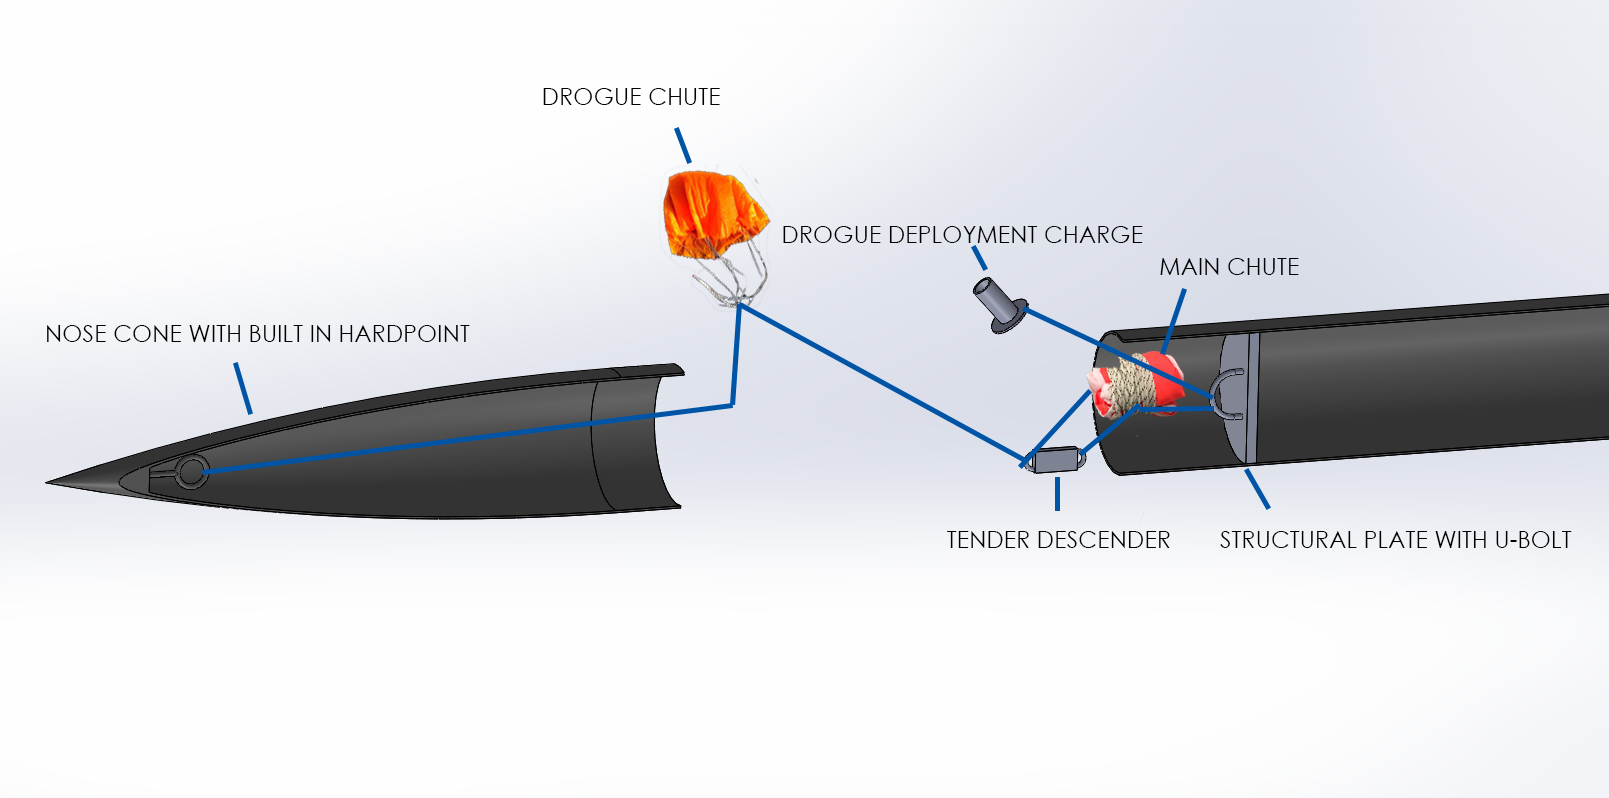
\includegraphics[scale=0.4]{imgs/recoverydetail.png}
    \caption{Exploded view of the Recovery system}
    \label{fig:recovery}
\end{figure}
\subsection{Ejection Charge} % (fold)
\label{sub:ejection_charge}
The ejection charge was held in a machined metal container attached to a wooden board. It rested above the main chute when packed into the rocket. Before flight, the container was filled with 10 grams of black powder and an e-match was wired to the avionics bay. The charge is attached to the forward body section with a nylon cord. 
\newline\newline
The size of the ejection charge (10 grams of black powder) is determined mathematically from first principles and tested rigorously and repeatedly on the ground with a 100\% success rate in the flight configuration. The black powder must provide a sufficient buildup of pressure to fracture three \#6-32 nylon bolts in shear. Calculating the failure loading of each bolt using published shear strength values, it was determined that a total of 228 pounds-force was required to separate all three bolts. The required pressure difference between the inside of the recovery bay and the atmosphere was then calculated, using the surface area given by the inner diameter of the recovery bay (6 inches). This total pressure difference (8 psi) represented the sum of the pressure caused by the black powder detonation and the change in pressure due to the altitude difference of approximately 11 000 feet, as a lower bound. The latter is approximately 5.8 psi, meaning that the black powder charge must be sufficient to generate at least 2.2 psi of pressure in the recovery bay. As verified by a black powder charge calculator online, using 10 grams of black powder is sufficient to ensure shearing of all shear pins on the ground (8 psi), which guarantees the shear threshold will be crossed even in the event of an air leak within the recovery bay.
\subsection{Tender Descender} % (fold)
\label{sub:tender_descender}
The Tender Descender is a commercially designed product designed for dual deployment in amateur rocketry. It consists of two carabiners held in place by a pin; this assembly is retained until a small charge (3 grams of black powder) releases the pin, freeing the carabiners. By attaching the top end of the main parachute to one carabiner and the bottom end of the parachute to the other carabiner (and the rocket body), deployment of the main parachute is achieved by sending a command to detonate the charge within the Tender Descender, separating the halves. Before flight, the tender descender was filled with black powder and an e-match was set in place, wired to the avionics bay. It is directly connected to the Stratologger module, which is programmed to issue the command to fire the charge at 700 feet AGL.
\subsection{Parachutes} % (fold)
\label{sub:parachutes}
Two parachutes were packed for a dual deployment recovery. Both parachutes are COTS parts manufactured by Fruity Chutes. The parachute sizes and models were chosen on the basis of terminal velocity (i.e. rate of descent at equilibrium). The drogue parachute should allow the rocket to adopt a safe, nose-up attitude and maintain this orientation until the main parachute is deployed, while preventing excessive transverse drifting due to wind conditions near the launch area. The main parachute should slow the rocket down to a safe speed for impact with terrain upon landing so that the rocket and its internal components remain undamaged. The drogue parachute was 15” in diameter, and the main parachute was 60” in diameter. Using the manufacturer’s listed drag coefficients and dimensions for each parachute, this configuration results in a projected terminal velocity of 31.41 m/s (103.05 ft/s) under the drogue chute and 7.85 m/s (25.75 ft/s) under the main chute.
\newline\newline
The drogue chute was packed into the nose cone and attached to the top of the main chute via a length of Kevlar shock cord and the Tender Descender, so that the drogue deployment event would allow the main parachute to be released but not inflated. It was also attached to an eye bolt at the tip of the nosecone, which provided a hard point against the shock loading during deployment. The base of the main parachute was attached to a U-bolt on the pressure bulkhead, serving as another hard point, and the top was secured to the Tender Descender. Both parachutes were wrapped using fire-resistant Nomex blankets to protect them from the black powder charge during the separation event.
\subsection{Avionics} % (fold)
\label{sub:avionics}
TODO